\documentclass[a4paper,12pt]{article}

% Packages
\usepackage[utf8]{inputenc}
\usepackage[english]{babel}
\usepackage{amsmath}
\usepackage{amssymb}
\usepackage{graphicx}
\usepackage{geometry}
\usepackage{float}
\usepackage{caption}
\usepackage{booktabs}
\usepackage{pdfpages}
\usepackage{hyperref}

% Page layout
\geometry{margin=1in}

% Title and Author
\title{Rakéták, rakéta hajtóművek\\ 1. házifeladat}
\author{Ábrók László Patrik\\ JPWF8N}
\date{2025.04.13.} % Date of submission
%\date{\today}

\begin{document}

% Title Page
\maketitle
%\tableofcontents
\newpage

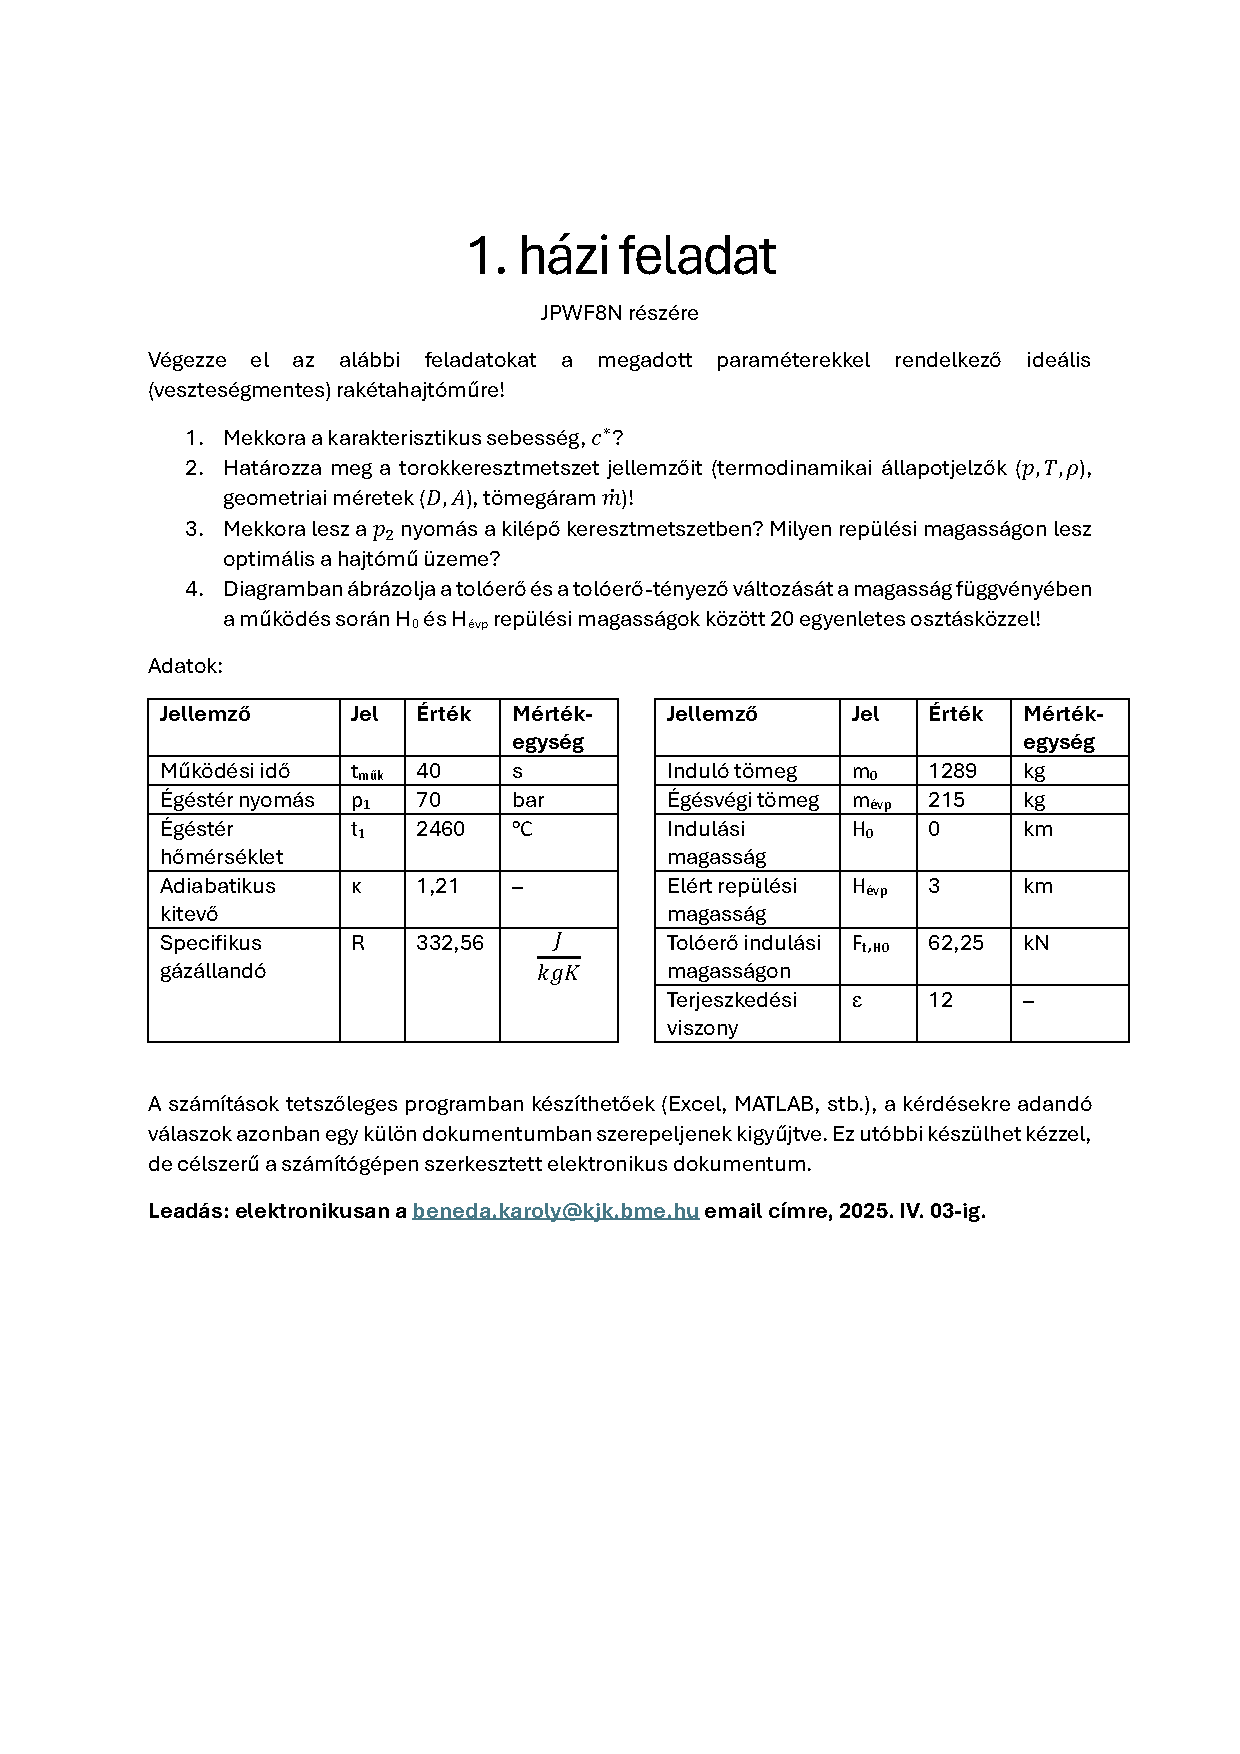
\includepdf[pages=-]{../handout/hw-1-JPWF8N.pdf}

% Section 1: Introduction
\section{Bevezetés}
A feladat elvégzéséhez a Python programozási nyelvet használtam. Az egyes kérdésekhez tartozó számításokat egy Jupyter notebook-ban vezettem le.
A megoldáshoz a következő könyvtárakat használtam:
\begin{itemize}
    \item \texttt{numpy} - numerikus számításokhoz
    \item \texttt{scipy} - közelítő megoldáshoz
    \item \texttt{matplotlib} - grafikonok készítéséhez
    \item \texttt{pandas} - adatok kezeléséhez
\end{itemize}
A megoldás megtalálható a következő GitHub repository-ban:
\href{https://github.com/LaszloAbrok/rockets-and-rocket-engines}{rockets-and-rocket-engines repository}

A notebook futtatásához célszerű egy virtuális környezet létrehozása, amelyben a szükséges könyvtárak telepítve vannak.
A szükséges könyvtárak elérhetőek egy requirements.txt fájlban, amelyet a következő paranccsal telepíthetünk:
\begin{verbatim}
pip install -r requirements.txt
\end{verbatim}

Az adatokat egy json fájlban tároltam, amelyet a notebookban beolvasok. A json fájl tartalma a következő:
\begin{verbatim}
    {
        "t_muk": 40,
        "p_1": 7000000,
        "t_1": 2733.15,
        "k": 1.21,
        "R": 332.56,
        "m_0": 1289,
        "m_evp": 215,
        "H_0": 0,
        "H_evp": 3000,
        "F_t_h0": 62250,
        "epsilon": 12
    }
\end{verbatim}

A feladatleírásban felsorolt mértékegységeket SI-ben adtam meg.

\section{Karakreterisztikus sebesség}
A karakterisztikus sebesség azt adja meg, hogy milyen hatékonyan képes a hajtómű
a hőenergiát mozási energiává alakítani. Ez a jellemző a torok méretétől és tömegáramtól függ.
\\Tömegáram kiszámítása:
\[
\dot{m} = \frac{m_0 - m_{\text{evp}}}{t_{\text{muk}}}
\]
\[
\dot{m} = \frac{1289 - 215}{40} = 26.85 \text{ kg/s}
\]
\\A torok méretének kiszámítása:
\[
A_t = \frac{\dot{m}}{p_1 \cdot \sqrt{\frac{k}{R \cdot T_1}} \cdot \left( \frac{2}{k+1} \right)^{\frac{k+1}{2(k-1)}}}
\]
\[
A_t = \frac{26.85}{7000000 \cdot \sqrt{\frac{1.21}{332.56 \cdot 2733.15}} \cdot \left( \frac{2}{1.21+1} \right)^{\frac{1.21+1}{2(1.21-1)}}} = 0.0056 m^2
\]
\\Karakterisztikus sebesség kiszámítása:
\[
c^* = \frac{p_1 \cdot A_t}{\dot{m}}
\]
\[
c^* = \frac{7000000 \cdot 0.0056}{26.85} = 1465.6904 \text{ m/s}
\]

\section{A torokkeresztmetszet jellemzői}
A tömegáram már az előző részben kiszámításra került.\\
A torokátmérő kiszámítása:
\[
d_t = \sqrt{\frac{4 \cdot A_t}{\pi}}
\]
\[
d_t = \sqrt{\frac{4 \cdot 0.0056}{\pi}} = 0.0846 \text{ m}
\]
Poisson egyenlet segítségével kiszmátható a toroknál mérhető hőmérséklet.
\[
T_t = \frac{2 \cdot T_1}{k + 1}
\]
\[
T_t = \frac{2 \cdot 2733.15}{1.21 + 1} = 2473.4389 \text{ K}
\]
Az izentropikus folyamat nyomása:
\[
p_t = p_1 \cdot \left( \frac{2}{k + 1} \right)^{\frac{k}{k - 1}}
\]
\[
p_t = 7000000 \cdot \left( \frac{2}{1.21 + 1} \right)^{\frac{1.21}{1.21 - 1}} = 3937755.2917 \text{ Pa} = 3937.7552917 \text{ kPa}
\]
Sűrűség:
\[
\rho_t = \frac{p_t}{R \cdot T_t}
\]
\[
\rho_t = \frac{3937755.2917}{332.56 \cdot 2473.4389} = 4.7872 \text{ kg/m}^3
\]

\section{Kilépő nyomás és optimális magasság}
A kilépő nyomás meghatározásához szükség van a kilépő Mach szám meghatározására. Ezt analaítikus módon nem lehet megoldani, ezért iteratív eljárását használtam. A következő egyenlet nem oldható meg zárt alakban:
\[
f(M) = \frac{1}{M} \cdot \left( \frac{2}{k+1} \left(1 + \frac{k-1}{2}M^2 \right) \right)^{\frac{k+1}{2(k-1)}} - \varepsilon
\]

Ezért a következő egyenletet oldottam meg gyökkereséssel:
\[
f(M_e) = 0 \quad \Rightarrow \quad \varepsilon = \frac{1}{M_e} \cdot \left( \frac{2}{k+1} \left(1 + \frac{k-1}{2}M_e^2 \right) \right)^{\frac{k+1}{2(k-1)}}
\]

A megoldáshoz a \textit{scipy} könyvtár \texttt{fsolve} függvényét használtam, 3.0 kezdeti értékkel.
Ennek eredménye:
\[
M_e = 3.4373
\]

Ezt követően a kilépő nyomás kiszámítása a következő egyenlet segítségével történik:
\[
p_2 = p_1 \cdot \left(1 + \frac{k - 1}{2} M_e^2 \right)^{-\frac{k}{k - 1}}
\]
\[
p_2 = 7000000 \cdot \left(1 + \frac{1.21 - 1}{2} \cdot 3.4373^2 \right)^{-\frac{1.21}{1.21 - 1}} = 67042.3800 \text{ Pa} = 67.0423800 \text{ kPa}
\]

Az optimális magasság meghatározásához azt vettem figyelembe, hogy egy hajtómű akkor működik a legoptimálisabban, ha a fúvókából kilépő nyomás megegyezik a külső nyomással.\\
A megoldáshoz a standard ISA modellt használtam, amely a következő egyenlettel írható le:

\[
p(h) = p_0 \left(1 - \frac{L \cdot h}{T_0} \right)^{\frac{g M}{R L}}
\]

Ebből kifejezve a magasságot:

\[
h_{opt} = \frac{T_0}{L} \left( 1 - \left( \frac{p_2}{p_0} \right)^{\frac{R L}{g M}} \right)
\]

A következő konstansokat használtam:

\[
\begin{array}{|c|c|c|}
\hline
\textbf{Jelölés} & \textbf{Érték} & \textbf{Mértékegység} \\
\hline
p_0 & 101325 & \text{Pa} \\
\hline
T_0 & 288.15 & \text{K} \\
\hline
L & 0.0065 & \text{K/m} \\
\hline
g & 9.81 & \text{m/s}^2 \\
\hline
M_{air} & 0.02896 & \text{kg/mol} \\
\hline
R & 8.31446 & \text{J/mol·K} \\
\hline
\end{array}
\]

\[
h_{opt} = \frac{288.15}{0.0065} \left( 1 - \left( \frac{67.0423800}{101325} \right)^{\frac{287.05 \cdot 0.0065}{9.81 \cdot 0.0289644}} \right) = 3349.6154 \text{ m}
\]

\section{Tolóerő és tolóerőtényező}
A tólóerő kiszámításához a tólóerő egyenletét használtam:

\[
F_t = \dot{m} \cdot w + (p_2 - p_0) \cdot A_2
\]

Ebből:
\[
w  = \frac{F_t - (p_2 - p_0) \cdot A_2}{\dot{m}}
\]

\[ w = \frac{62250 - (67042.3800 - 101325) \cdot 0.0675}{26.85} = 2404.5747 \text{ m/s} \]

A kilépő sebesség segítségével minden egyes vizsgált magasságra kiszámítottam a tolóerőt a tolóerő egyentlet segítségével.
A nyomás adott magasságon történő meghatározásához a következő egyenletet használtam fel:
\[ p = p_0 \left(1 - \frac{T_0 L h}{R L g M}\right)^{\frac{g M}{R L}} \]
A tolóerőtényezőket pedig a következő összefüggéssel számoltam:
\[
c_f = \frac{F_t}{p_1 \cdot A_t}
\]
A következő ábrán látható a tolóerő és tolóerőtényező változása a magassággal 0 és 3000 méter között 20 osztásközzel:
\begin{figure}[H]
    \centering
    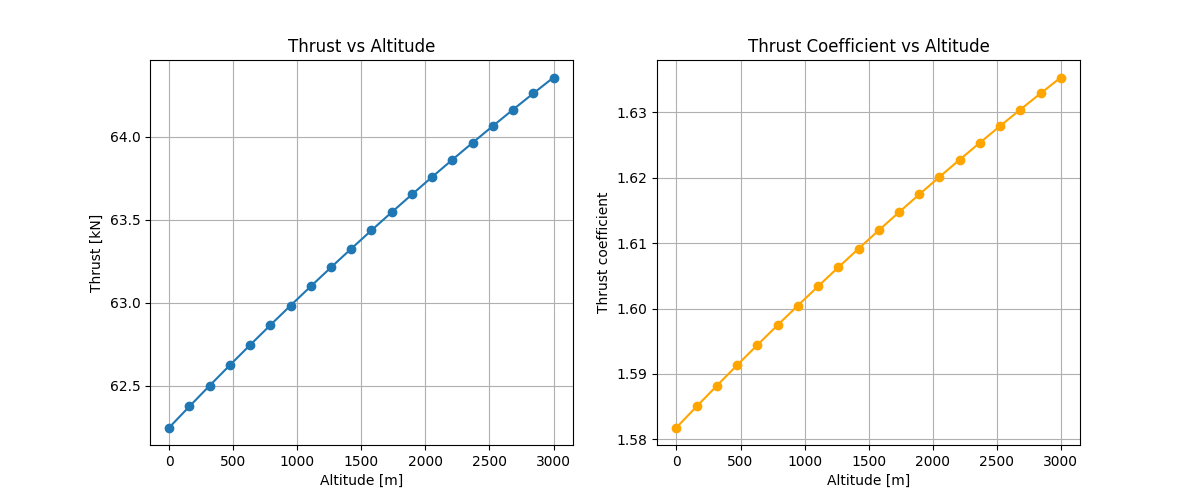
\includegraphics[width=1\textwidth]{images/plots.png}
    \caption{Tolóerő és tolóerőtényező változása a magassággal}
    \label{fig:rocket_force}
\end{figure}

A következő táblázat pedig tartalmazza az egyes magasságokhoz tartozó tolóerőt és tolóerőtényezőt.
\[
\begin{array}{|c|c|c|}
\hline
\textbf{Magasság [m]} & \textbf{Tolóerő [kN]} & \textbf{Tolóerőtényező} \\
\hline
0.0 & 62.25 & 1.5818 \\
157.89 & 62.38 & 1.5850 \\
315.79 & 62.50 & 1.5882 \\
473.68 & 62.63 & 1.5913 \\
631.58 & 62.75 & 1.5944 \\
789.47 & 62.87 & 1.5975 \\
947.37 & 62.98 & 1.6005 \\
1105.26 & 63.10 & 1.6034 \\
1263.16 & 63.21 & 1.6063 \\
1421.05 & 63.33 & 1.6091 \\
1578.95 & 63.44 & 1.6120 \\
1736.84 & 63.55 & 1.6147 \\
1894.74 & 63.65 & 1.6174 \\
2052.63 & 63.76 & 1.6201 \\
2210.53 & 63.86 & 1.6228 \\
2368.42 & 63.96 & 1.6254 \\
2526.32 & 64.06 & 1.6279 \\
2684.21 & 64.16 & 1.6304 \\
2842.11 & 64.26 & 1.6329 \\
3000.0 & 64.36 & 1.6353 \\
\hline
\end{array}
\]
\end{document}